\documentclass{article}
\usepackage[utf8]{inputenc}
\usepackage[left=2.5cm, right=2.5cm, top=2.5cm]{geometry}
\usepackage{amsmath,amssymb}
\usepackage{hyperref}
\usepackage{graphicx}
\newcommand{\nv}{\hat{\bf n}}
\title{tSZ $\times$ galaxies}
\date{\today}
\newcommand{\aj}    {{\em Astron.\ J.}}
\newcommand{\aap}{{\em Astron.\ Astrophys.}}
\newcommand{\apj}{{\em Astrophys.\ J.}}
\newcommand{\apjl}{{\em Astrophys.\ J.\ Lett.}}
\newcommand{\apjs}{{\em Astrophys.\ J.\ Suppl.}}
\newcommand{\mnras}{{\em Mon.\ Not.\ R.\ Astron.\ Soc.}}
\newcommand{\npb}{{\em Nucl.\ Phys.\ B}}
\newcommand{\nat}{{\em Nature}}
\newcommand{\physrep}{{\em Phys.\ Rep.}}
\newcommand{\pasj}{{\em Publ.\ Astron.\ Soc.\ Japan}}
\newcommand{\pasp}{{\em Publ.\ ASP}}
\newcommand{\jcap}{{\em J.\ Cosmol.\ Astropart.\ Phys.}}
\newcommand{\prd}{{\em Phys.\ Rev.\ D}}
\newcommand{\prl}{{\em Phys.\ Rev.\ Lett.}}
\newcommand{\procspie}{Proceedings of the SPIE}


\begin{document}
\maketitle

\section{Introduction}
  The aim of the project is to model and measure the cross power spectrum of the galaxy overdensity and the thermal Sunyaev-Zel'dovich effect.
  \begin{equation}
    \langle a^g_{\ell m} a^{y*}_{\ell' m'} \rangle=C^{gy}_\ell\,\delta_{\ell\ell'}\delta_{mm'}
  \end{equation}

  The kind of science we expect to extract from this is:
  \begin{enumerate}
    \item A tomographic measurement of the hydrostatic bias affecting tSZ cluster studies.
    \item More in general, we may be able to phrase that as a tomographic measurement of the different contributions to the total tSZ signal from different redshifts.
    \item From the 1-halo term we may be able to extract information about scatter between galaxy content and pressure in clusters (?).
  \end{enumerate}

\section{Theory modelling}
  The tSZ signal caused by a given structure is related to the projected gas pressure, $P_e(\hat{n} \chi)$, along our line of sight. For convenience, we work in units of comoving distance $\chi$, in which the Compton $y$ parameter is given by
  \begin{equation}
    y(\nv) = \frac{\sigma_T}{m_e c^2} \int \frac{d\chi}{1+z}\,P_e(\chi\nv),
  \end{equation}
  where $\sigma_T$ is the Thomson scattering cross section.

  The projected overdensities of galaxy number counts are related to the 3D number density fluctuations through a Kernel given by the redshift distribution of those galaxies
  \begin{equation}
    \delta_g(\nv) = \int d\chi\frac{dN_g}{d\chi} \Delta_g(\chi\nv).
  \end{equation}

  \subsection{Angular power spectra}
    In general, let's consider two projected quantities $u(\nv)$ and $v(\nv)$, related to three-dimensional fields $U({\bf r})$ $V({\bf r})$:
    \begin{equation}
      u(\nv)=\int d\chi\,W_u(\chi)\,U(\chi\nv),\hspace{12pt} v(\nv)=\int d\chi\,W_v(\chi)\,V(\chi\nv),
    \end{equation}
    where $W_{u,v}$ are their corresponding radial window functions.

    The angular power spectrum of the projected quantities can be related to the 3D power spectrum of the non-projected ones $P_{UV}$ as\footnote{Note that the expression above for $C_\ell^{uv}$ only holds in the \emph{Limber approximation}, and the exact expression would be
    \begin{equation}
      C^{uv}_\ell=\frac{2}{\pi}\int dk\,k^2 \int d\chi_1\,W_u(\chi_1)j_\ell(k\chi_1)\int d\chi_2\,W_u(\chi_2)j_\ell(k\chi_2)\,P_{UV}(\chi_1,\chi_2,k),
    \end{equation}
    where we $j_\ell$ are the spherical Bessel functions. The Limber approximation is appropriate for our purposes.}:
    \begin{equation}
      C_\ell^{uv} = \int \frac{dz}{H(z)} \frac{W_u(z)W_v(z)}{\chi^2(z)}\,P_{UV}\left( z, k=\frac{\ell+1/2}{\chi(z)} \right).
    \end{equation}
    Here, the 3D power spectrum is analogously defined as the variance of the Fourier-space 3D quantities:
    \begin{equation}
      \left\langle U({\bf k})V^*({\bf k}')\right\rangle = (2\pi)^3\,\delta({\bf k}-{\bf k}')\,P_{UV}(k).
    \end{equation}

    Using this notation, the window functions associated with the galaxy number overdensity and the tSZ anisotropy are simply:
    \begin{equation}
      W_g(\chi)=\frac{dN_g}{d\chi}=\frac{H(z)}{c}\,\frac{dN_g}{dz},\hspace{12pt}W_y(\chi)=\frac{\sigma_T}{m_ec^2}\frac{1}{1+z},
    \end{equation}
    where $H(z)$ is the expansion rate.


  \subsection{Halo model}
    We will use the halo model prescription for the 3D power spectrum. Let $U(r|M)$ and $V(r|M)$ be the profile of the two fields described above as a function of the comoving distance $r$ to the centre of a halo of mass $M$, and let us define the Fourier-space profiles simply as the Fourier transform of these:
    \begin{equation}
      U(k|M)\equiv4\pi \int_0^\infty dr\,r^2\,\frac{\sin(kr)}{kr}U(r|M)
    \end{equation}
    (and analogously for $V$).

    The halo model prediction for the cross-power spectrum $P_{UV}$ then consists of two contributions, from the so-called 1-halo term and 2-halo term:
    \begin{equation}
      P_{UV}(k)=P^{1h}_{UV}(k)+P^{2h}_{UV}(k).
    \end{equation}
    Each of these can be estimated in terms of the Fourier-space profiles as:
    \begin{align}
      &P^{1h}_{UV}(k)=\int dM\,\frac{dn}{dM}\,\langle U(k|M)\,V(k|M)\rangle\\
      &P^{2h}_{UV}(k)=P_L(k)\,\left[\int dM\frac{dn}{dM}\,b_h(M)\,\langle U(k|M)\rangle\right]\,\left[\int dM\frac{dn}{dM}\,b_h(M)\,\langle V(k|M)\rangle\right].
    \end{align}
    Here, $P_L(k)$ is the linear matter power spectrum, $dn/dM$ is the halo mass function and $b_h(M)$ is the halo bias. Further details are discussed in Appendix \ref{app:hm}.

  \subsection{Model specifics}
    \subsubsection{Cosmological quantities}
      We will use the linear power spectrum computed from CLASS (as provided by the Core Cosmology Library - CCL). We will use the Tinker 2010 mass function and halo bias \cite{2010ApJ...724..878T}, also provided by CCL. Distance-redshift relations etc. will also be produced by CCL

    \subsubsection{Halo profiles}
      We will use prescriptions for the halo profiles from the following references:
      \begin{itemize}
        \item {\bf Pressure.} For the time being we will stick to the choice of profile used by Planck (the GNFW ``Arnaud'' profile \cite{2010A&A...517A..92A,2016A&A...594A..24P}. This profile takes the form:
              \begin{equation}
                P_e(r)=P_*\,p(r/R_{500c}),
              \end{equation}
              where $r_{R00c}$ is the cluster radius enclosing an overdensity of 500 times the critical density (see Appendix \ref{app:massdef}). The normalization $P_*$ is given by
              \begin{equation}
                P_*=6.41\,\left(1.65 {\rm eV}\,{\rm cm}^{-3}\right)\left(\frac{h}{0.7}\right)^{8/3}\left(\frac{(h/0.7)(1-b)M_{500c}}{3\times10^{14}M_\odot}\right)^{2/3+0.12}
              \end{equation}
              and the form factor is
              \begin{equation}
                p(x)=(c_{500}x)^{-\gamma}\left[1+(c_{500}x)^\alpha\right]^{(\gamma-\beta)/\alpha},\hspace{12pt}(\alpha,\beta,\gamma,c_{500})=(1.33,4.13,0.31,1.81).
              \end{equation}
              
              We may also want to give the Battaglia et al. profile a go \cite{2012ApJ...758...75B}.
        \item {\bf Matter density} (useful for CMB lensing). We will use a truncated Navarro-Frenk and White (NFW) profile \cite{1997ApJ...490..493N}. See \cite{2017MNRAS.470.2100K} for further details on implementation.
              For a given mass definition $M_\Delta$ (see Appendix \ref{app:massdef}), the profile can be written as:
              \begin{equation}
                \rho(r)=M_\Delta u_m(r/r_\Delta),
              \end{equation}
              where
              \begin{equation}
                u_m(x)=\frac{c_\Delta^3}{4\pi\,r_\Delta^3\,[\log(1+c_\Delta)-c_\Delta/(1+c_\Delta)]}\,\frac{1}{c_\Delta x\,(1+c_\Delta x)^2}.
              \end{equation}
              The Fourier-space profile can be computed analytically (under the assumption that the profile is truncated at $r=r_\Delta$):
              \begin{align}\nonumber
                u_m(k)=\left[\log(1+c_\Delta)-\frac{c_\Delta}{(1+c_\Delta)}\right]^{-1}&\left[\cos(q)\left({\rm Ci}((1+c_\Delta)q)-{\rm Ci}(q)\right)\right.\\\nonumber
                      &\left.+\sin(q)\left({\rm Si}((1+c_\Delta)q)-{\rm Si}(q)\right)\right.\\&\left.-\sin(c_\Delta q)/(1+c_\Delta q)\right]
              \end{align}
              where $q\equiv kr_\Delta/c_\Delta$.
        \item {\bf Galaxy overdensity}. We will use a Halo Occupation Distribution as prescribed by \cite{2005ApJ...633..791Z,2011ApJ...736...59Z}. See implementation details in \cite{2017MNRAS.470.2100K}.
              We will model the galaxy content of dark matter halos as being made up of central and satellite galaxies. Centrals lie at the center of the halo, while satellites are distributed according to a profile $u_s(r)$. Halos can have zero or one central, and the mean number of centrals for a halo of mass $M$ is modelled as a smoothed step function
              \begin{equation}
                \langle N_c(M)\rangle=\frac{1}{2}\left[1+{\rm erf}\left(\frac{\log(M/M_{\rm min})}{\sigma_{\rm lnM}}\right)\right].
              \end{equation}
              We then assume that satellites can only be formed if a halo has a central and has a mass larger than some threshold $M_0$. In that case, average number of satellites is a power law of the form:
              \begin{equation}
                \langle N_s(M)\rangle=\Theta(M-M_0)\,\left(\frac{M-M_0}{M_1'}\right)^{\alpha_s}.
              \end{equation}
              Furthermore, we may assume that only a fraction $f_c$ of centrals make it into our selection.

              Putting everything together, the galaxy overdensity profile is given by:
              \begin{equation}
                u_g(k|M)=\bar{n_g}^{-1}\langle N_c(M)\rangle\left[f_c+\langle N_s(M)\rangle\,u_s(k|M)\right],
              \end{equation}
              where the number density of galaxies is
              \begin{equation}
                \bar{n}_g\equiv\int dM\,\frac{dn}{dM}\langle N_c(M)\rangle\left[f_c+\langle N_s(M)\rangle\right].
              \end{equation}
              Finally, for simplicity we will assume that the satellites follow the matter distribution: $u_s(k|M)=u_m(k|M)$ (i.e. an NFW profile).
        \item 1-halo covariance: note that different halo properties are not perfectly correlated due to e.g. hidden variables (age, merger history, environment etc.). I.e. in almost all cases
              \begin{equation}
                \langle U(k|M) V(k|M)\rangle\neq\langle U(k|M)\rangle\langle V(k|M)\rangle.
              \end{equation}
              In the particular case of the cross-correlation between tSZ flux and galaxy overdensity, we will model the scatter between both quantities by introducing one additional parameter $\rho_{yg}$:
              \begin{equation}
                \langle u_g(k) u_y(k)\rangle = (1+\rho_{yg})\langle u_g(k)\rangle \langle u_y(k)\rangle.
              \end{equation}
      \end{itemize}
      For the moment we will only consider the following four free parameters: $M_{\rm min}$, $M_1$, $1-b$, $\rho_{yg}$. We will fix all other parameters to the following values: $M_0=M_{\rm min}$, $\sigma_{{\rm ln}M}=0.15$, $\alpha=1$, $f_c=1$. We will fix cosmological parameters to the latest Planck values.

\section{Measurement}
  \subsection{Data}
    \begin{itemize}
      \item {\bf Galaxies:} For the moment we've used only maps of the galaxy overdensity field for the 2MPZ sample and the 5 WISC redshift bins. We'll see what we do with SDSS later on. We're also using the redshift distribution for these samples that were estimated in the CMB lensing cross-correlation paper. We use the masks provided.
      \item {\bf tSZ:} We've downloaded the tSZ MILCA and NILC maps. For these we use the Planck 60\% foreground mask.      
    \end{itemize}

  \subsection{Power spectra}
    We compute unbiased angular power spectra using {\tt NaMaster}, a well-tested pseudo-$C_\ell$ code \cite{2019MNRAS.484.4127A}. We have computed all auto- and cross-spectra between maps, but so far we have only analyzed the auto-correlation of the galaxy overdensities from 2MPZ and MILCA, and their cross-correlation with the MILCA $y$ map.

  \subsection{Covariance matrix}
    We compute three versions of the covariance matrix:
    \begin{enumerate}
      \item {\bf Theoretical covariance.} We estimate this covariance as a sum of two terms: the Gaussian disconnected part and the 1-halo connected trispectrum.
            \begin{itemize}
              \item Gaussian disconnected covariance: we use the approach of \cite{2004MNRAS.349..603E}, which fully accounts for the effects of mode coupling from survey geometry.
              \item 1-halo trispectrum: this is computed as
                    \begin{equation}\nonumber
                       {\rm Cov}(C^{uv}_\ell,C^{xy}_{\ell'})=\frac{1}{4\pi f_{\rm sky}}\int {d\chi}{\chi^2}\frac{W^u(\chi)W^v(\chi)W^x(\chi)W^y(\chi)}{\chi^4}\left\langle U(k|M)V(k|M)X(k'|M)Y(k'|M)\right\rangle,
                    \end{equation}
                    where $k=(\ell+1/2)/\chi$ and $k'=(\ell'+1/2)/\chi$.
            \end{itemize}
            Note that this covariance requires a model for the power spectra and halo profiles. We obtain these from the best-fit model found using a purely Gaussian covariance for which we use, as a model, an interpolated version of the power spectra measured from the data.
      \item {\bf Jackknife covariance.} We produce a set of 460 jackknife maps produced by removing patches corresponding to $N_{\rm side}=8$ HEALPix pixels. We only take pixels that are more than half unmasked.
      \item {\bf Combined covariance.} The reduced number of jackknife regions makes the jackknife noisy, and its inverse a bit unstable. To remedy this we combine the two covariances above as follows:
            \begin{itemize}
              \item We take the diagonal of the combined covariance to be the maximum of the jackknife and theory covariances. Note that this only matters at low $\ell$, where the jackknife covariance underestimates the uncertainties.
              \item We estimate the correlation matrix (i.e. $r_{ij}\equiv{\rm Cov}_{ij}/\sqrt{{\rm Cov}_{ii}{\rm Cov}_{jj}}$) from the theoretical covariance. This is to ensure that we have a smooth correlation structure, which we know should be well captured by the theoretical approach used here.
              \item We combine diagonals and correlation matrix into the final covariance matrix.
            \end{itemize}
    \end{enumerate}
  
  \subsection{Likelihood}
    We assume a Gaussian likelihood $-2\log{\cal L}=({\bf d}-{\bf t})^T{\sf C}^{-1}({\bf b}-{\bf t})$, where ${\bf d}$ is a data vector formed by stacking a series of power spectrum measurements, ${\bf t}$ is the corresponding vector of theory predictions and ${\sf C}$ is the covariance matrix described above.
    
    We analyse each redshift bin independently in order to limit the size of the data vector and the corresponding covariance. Thus, in each case the data vector is constructed by stacking two power spectrum measurements ${\bf d}=(\vec{C}^{gg}_\ell,\vec{C}^{gy}_\ell)$.
    
    We impose scale cuts to avoid having to model very non-linear scales. We limit ourselves to a maximum wavenumber $k_{\rm max}=1\,{\rm Mpc}^{-1}$, which we map into a maximum multipole $\ell_{\rm max}=k_{\rm max}\chi(\bar{z})-1/2$, where $\bar{z}$ is the mean redshift of each redshift bin.

\section{Results}
  Results for 2MPZ and the 5 WISC redshift bins in Figures \ref{fig:res_2mpz}, \ref{fig:res_wisc1}, \ref{fig:res_wisc2}, \ref{fig:res_wisc3}, \ref{fig:res_wisc4} and \ref{fig:res_wisc5} respectively. Results are summarized in Fig. \ref{fig:oneminusb}.
  \begin{figure*}
    \centering
    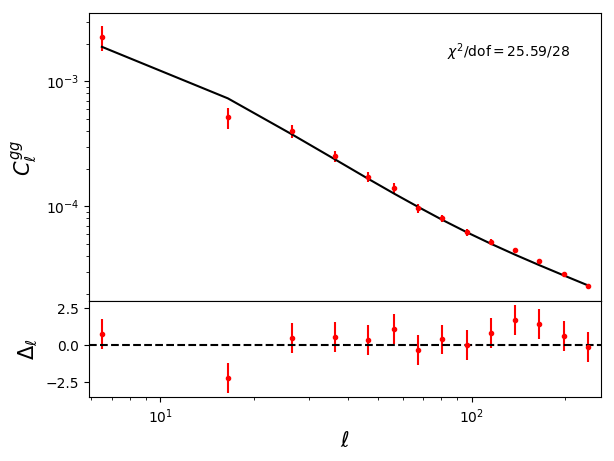
\includegraphics[width = 0.49\textwidth]{../output_test/sampler_minimal_hmc_2mpz_cls_2mpz_2mpz}
    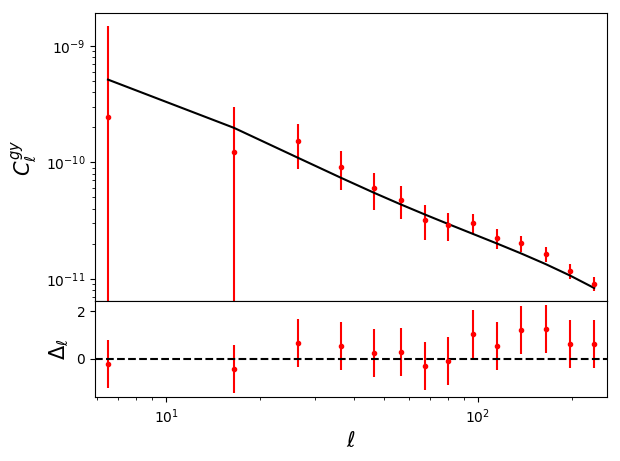
\includegraphics[width = 0.49\textwidth]{../output_test/sampler_minimal_hmc_2mpz_cls_2mpz_y_milca}
    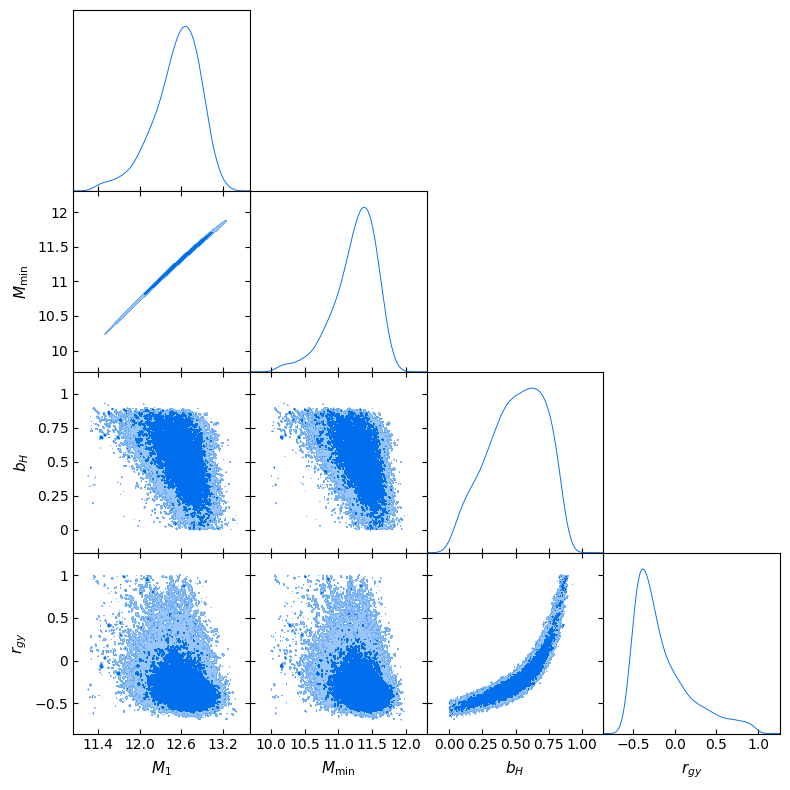
\includegraphics[width = 0.90\textwidth]{../output_test/sampler_minimal_hmc_2mpz_triangle}
    \caption{{\sl Upper left:} galaxy-galaxy power spectrum. {\sl Upper right:} galaxy-tSZ power spectrum. {\sl Lower:} parameter constraints. All for the 2MPZ sample.}\label{fig:res_2mpz}
  \end{figure*}
  \begin{figure*}
    \centering
    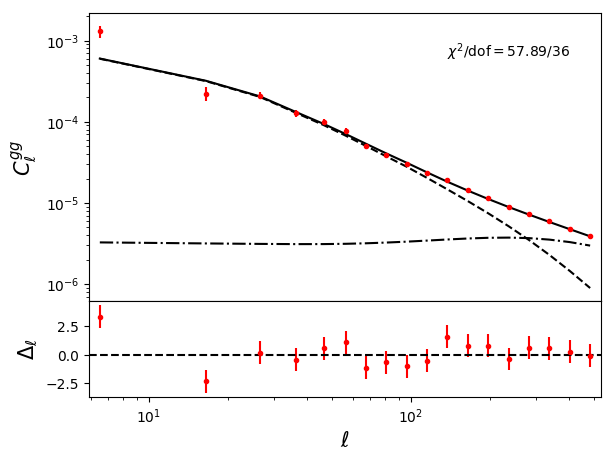
\includegraphics[width = 0.49\textwidth]{../output_test/sampler_minimal_hmc_wisc1_cls_wisc1_wisc1}
    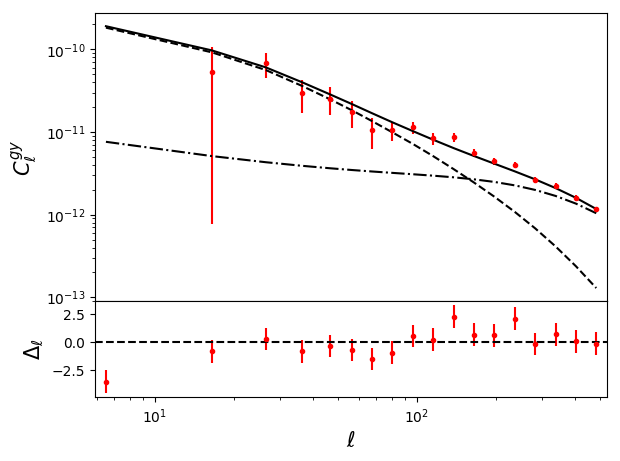
\includegraphics[width = 0.49\textwidth]{../output_test/sampler_minimal_hmc_wisc1_cls_wisc1_y_milca}
    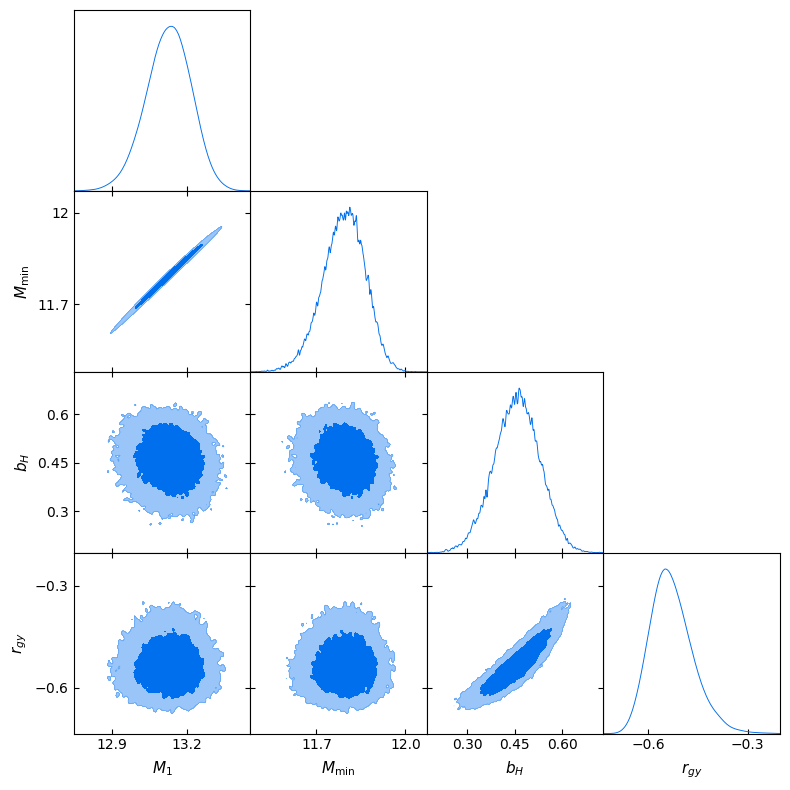
\includegraphics[width = 0.90\textwidth]{../output_test/sampler_minimal_hmc_wisc1_triangle}
    \caption{Same as Fig. \ref{fig:res_2mpz} for the first WISC bin.}\label{fig:res_wisc1}
  \end{figure*}
  \begin{figure*}
    \centering
    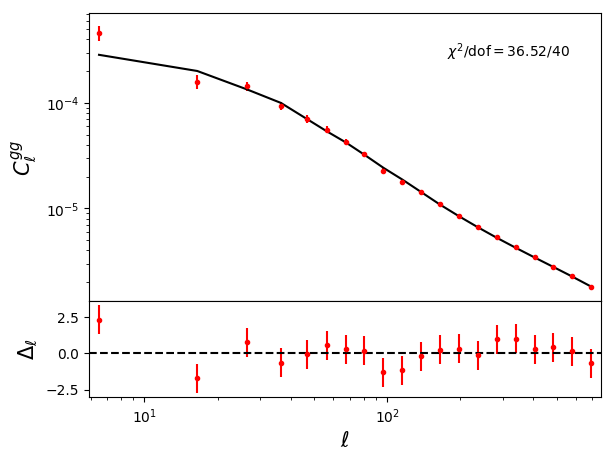
\includegraphics[width = 0.49\textwidth]{../output_test/sampler_minimal_hmc_wisc2_cls_wisc2_wisc2}
    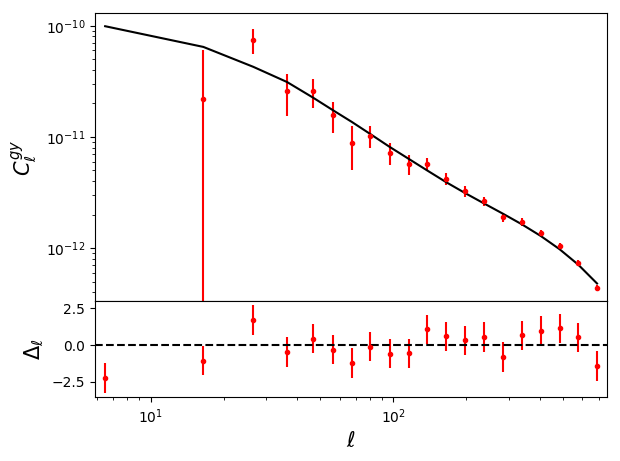
\includegraphics[width = 0.49\textwidth]{../output_test/sampler_minimal_hmc_wisc2_cls_wisc2_y_milca}
    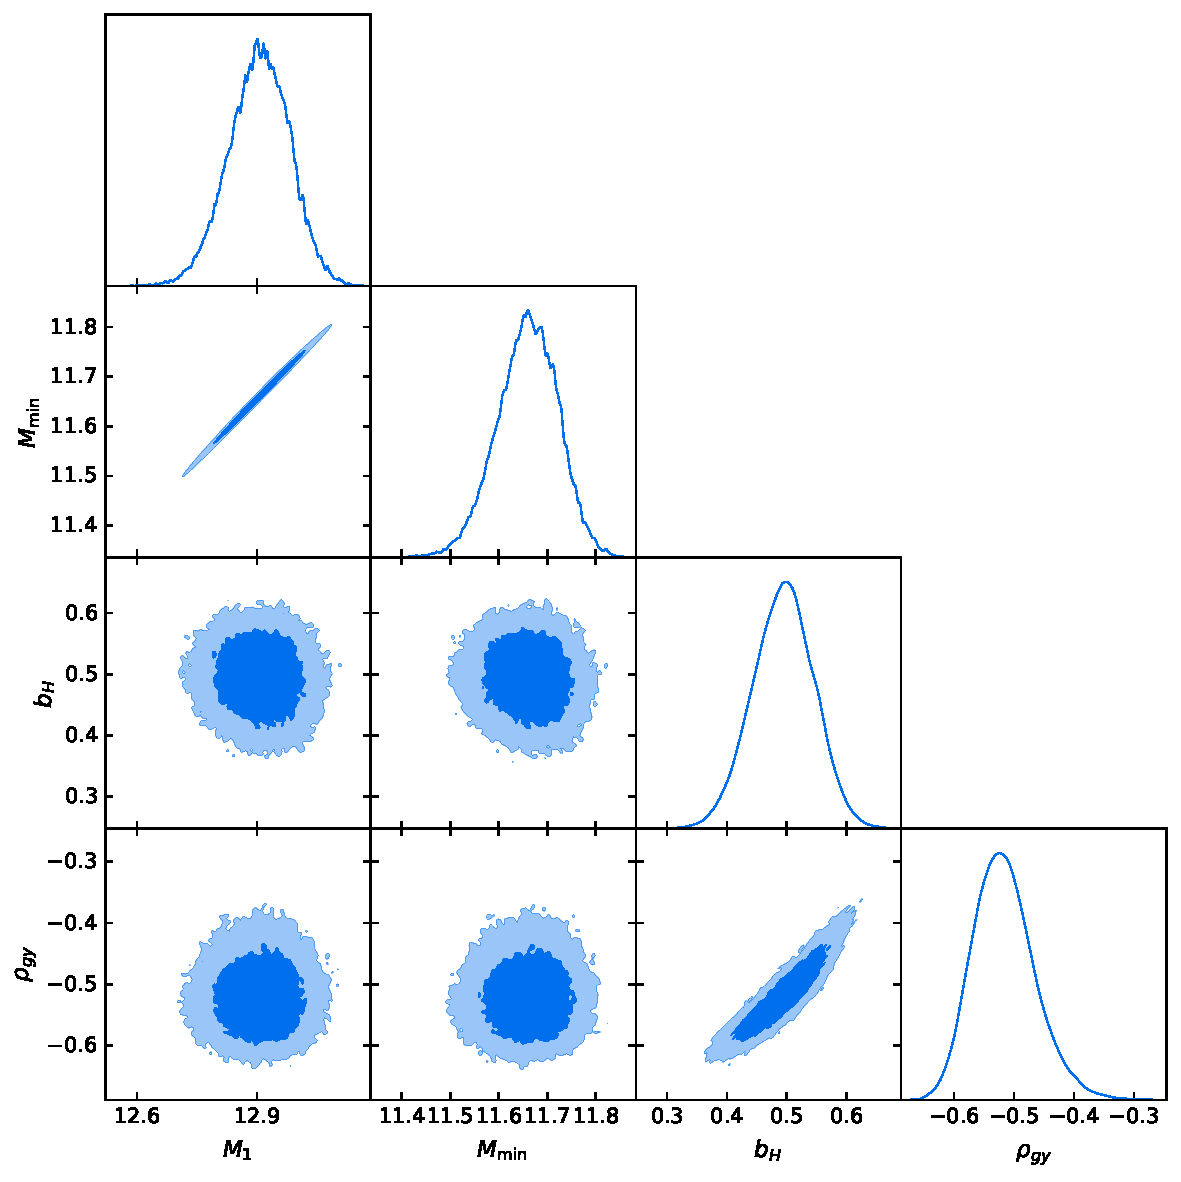
\includegraphics[width = 0.90\textwidth]{../output_test/sampler_minimal_hmc_wisc2_triangle}
    \caption{Same as Fig. \ref{fig:res_2mpz} for the second WISC bin.}\label{fig:res_wisc2}
  \end{figure*}
  \begin{figure*}
    \centering
    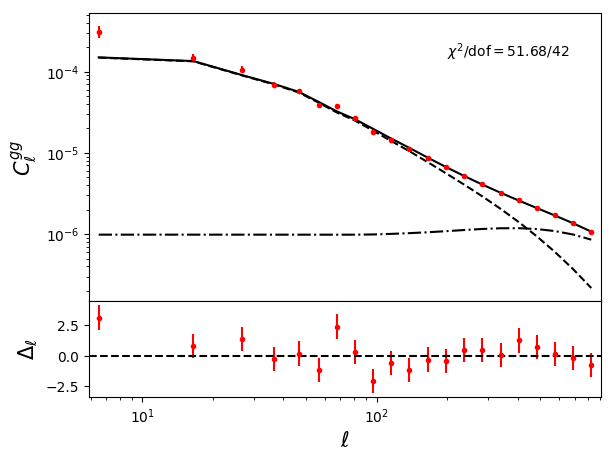
\includegraphics[width = 0.49\textwidth]{../output_test/sampler_minimal_hmc_wisc3_cls_wisc3_wisc3}
    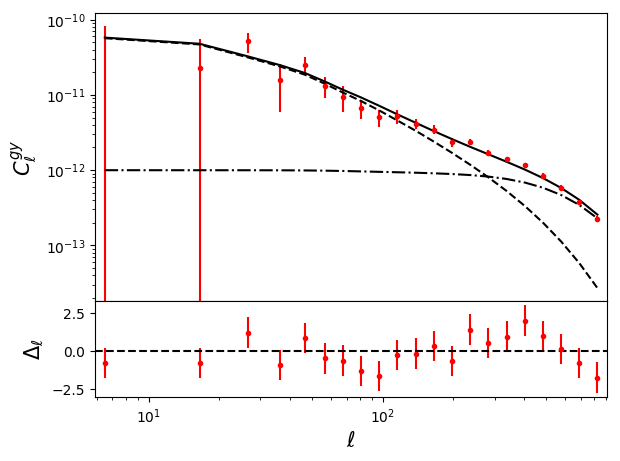
\includegraphics[width = 0.49\textwidth]{../output_test/sampler_minimal_hmc_wisc3_cls_wisc3_y_milca}
    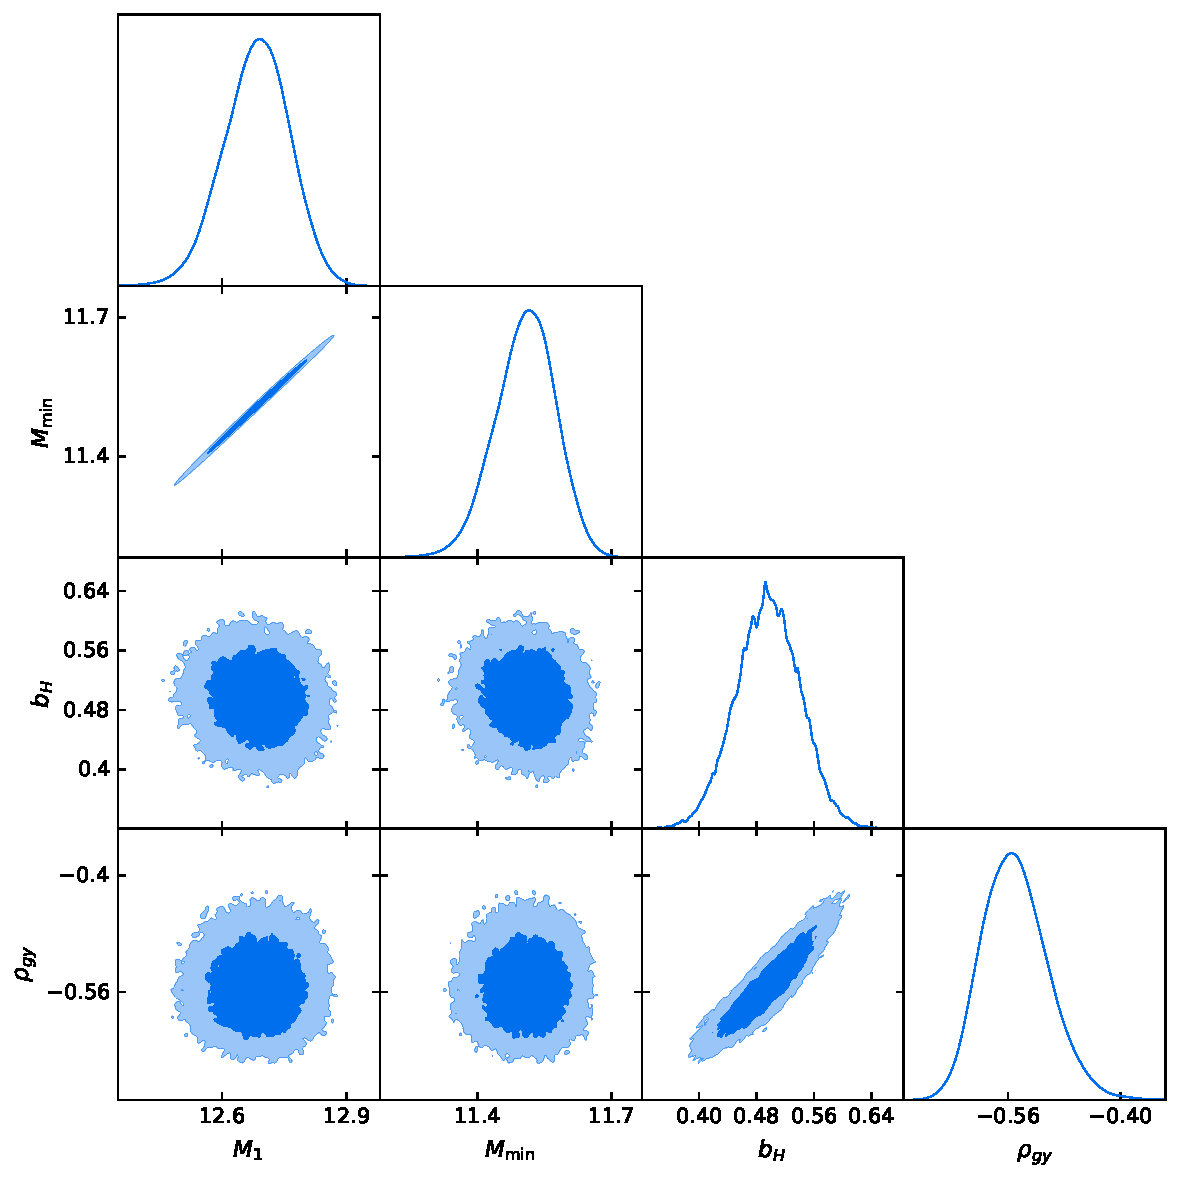
\includegraphics[width = 0.90\textwidth]{../output_test/sampler_minimal_hmc_wisc3_triangle}
    \caption{Same as Fig. \ref{fig:res_2mpz} for the third WISC bin.}\label{fig:res_wisc3}
  \end{figure*}
  \begin{figure*}
    \centering
    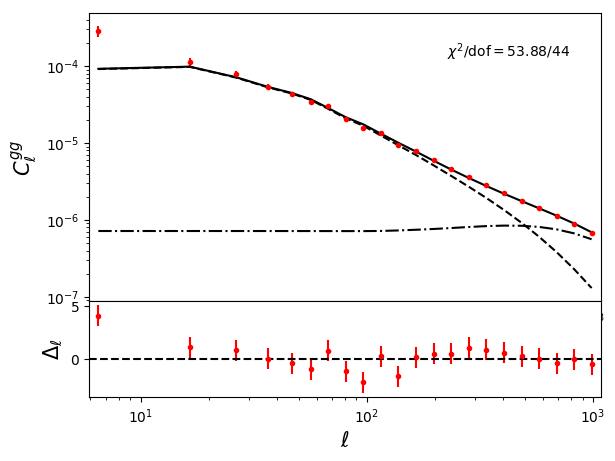
\includegraphics[width = 0.49\textwidth]{../output_test/sampler_minimal_hmc_wisc4_cls_wisc4_wisc4}
    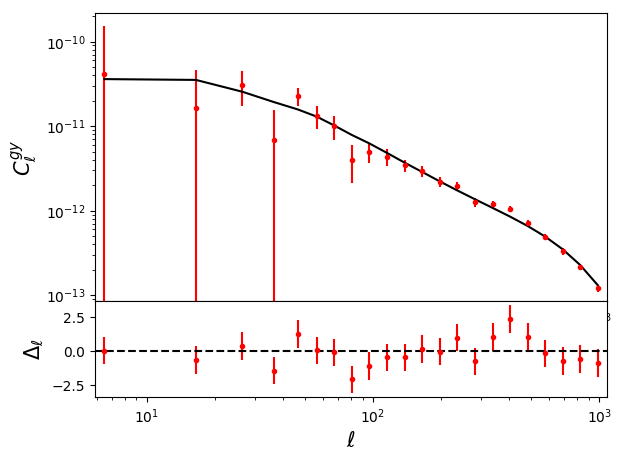
\includegraphics[width = 0.49\textwidth]{../output_test/sampler_minimal_hmc_wisc4_cls_wisc4_y_milca}
    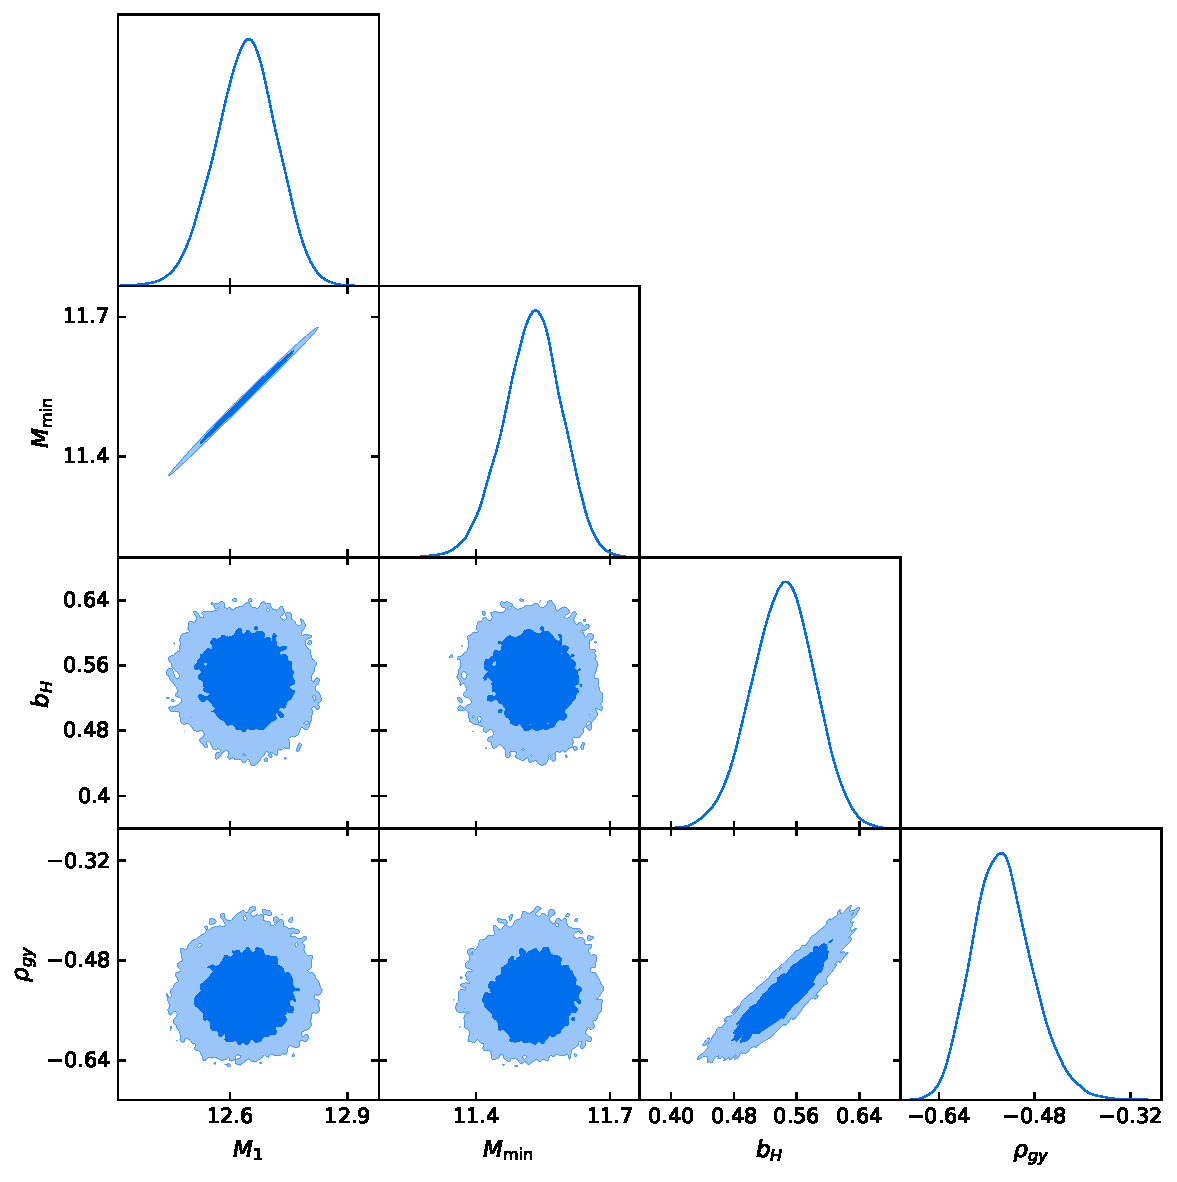
\includegraphics[width = 0.90\textwidth]{../output_test/sampler_minimal_hmc_wisc4_triangle}
    \caption{Same as Fig. \ref{fig:res_2mpz} for the fourth WISC bin.}\label{fig:res_wisc4}
  \end{figure*}
  \begin{figure*}
    \centering
    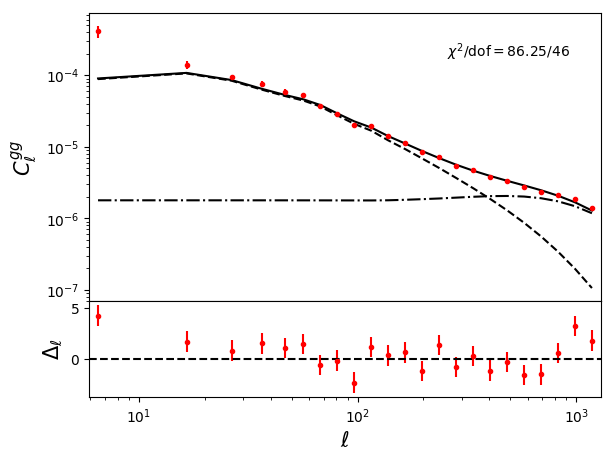
\includegraphics[width = 0.49\textwidth]{../output_test/sampler_minimal_hmc_wisc5_cls_wisc5_wisc5}
    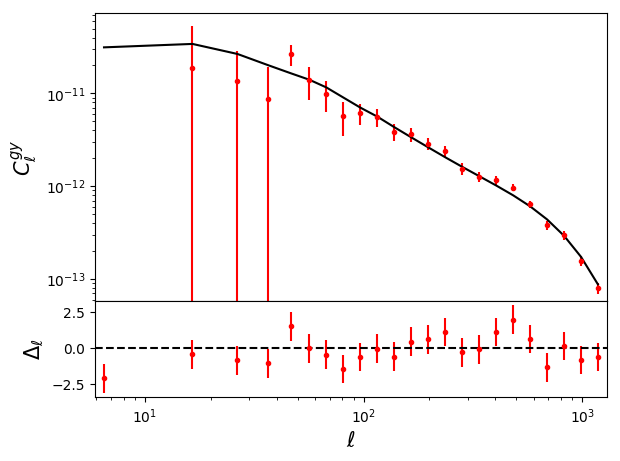
\includegraphics[width = 0.49\textwidth]{../output_test/sampler_minimal_hmc_wisc5_cls_wisc5_y_milca}
    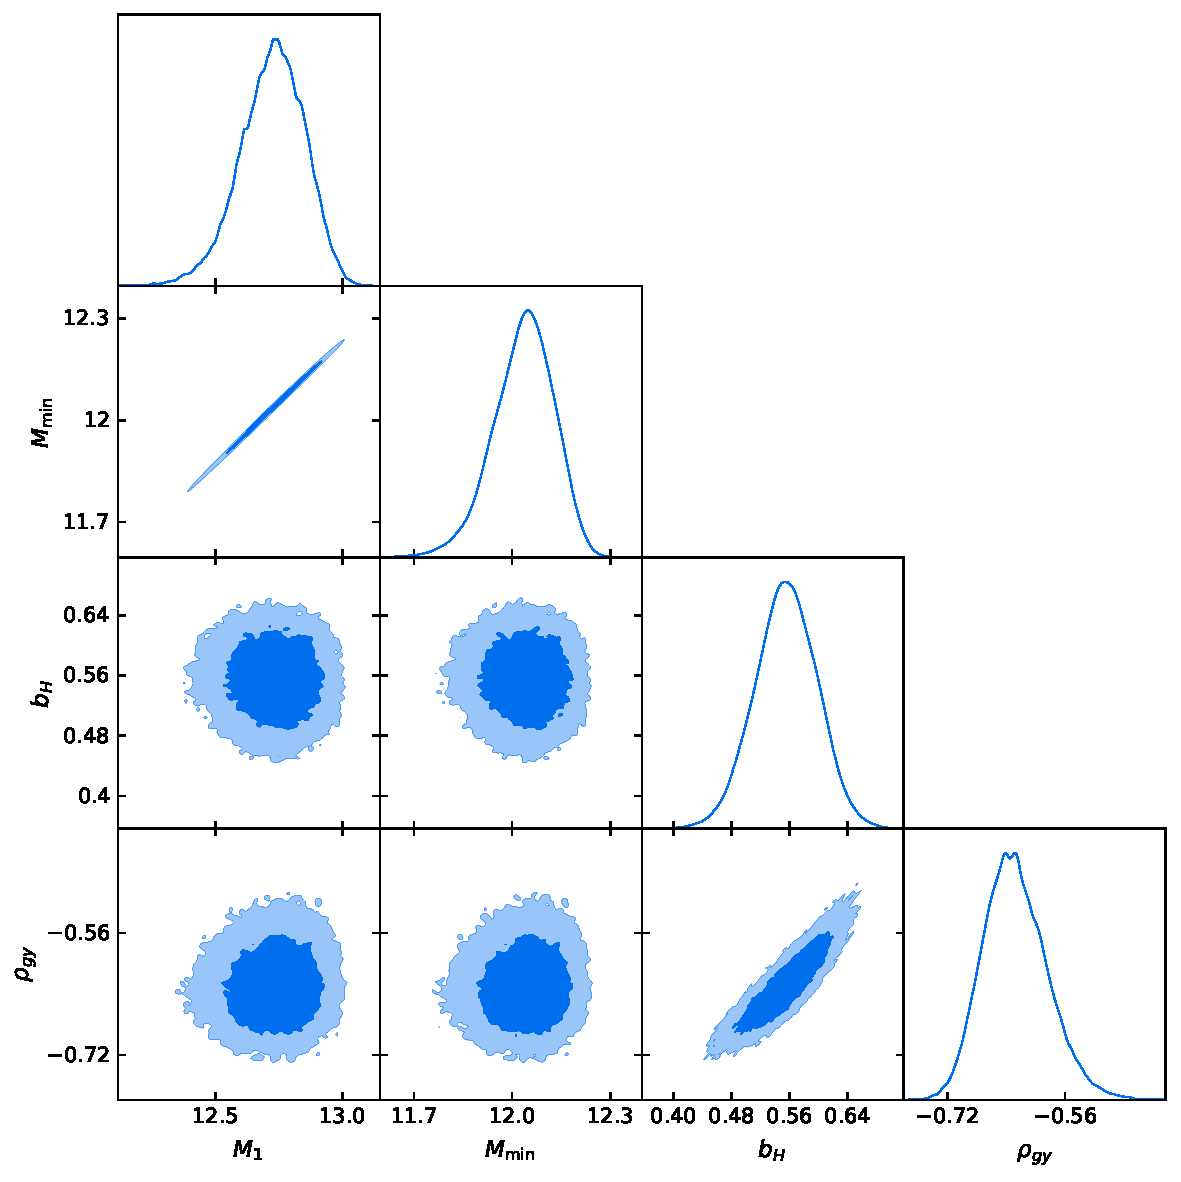
\includegraphics[width = 0.90\textwidth]{../output_test/sampler_minimal_hmc_wisc5_triangle}
    \caption{Same as Fig. \ref{fig:res_2mpz} for the fifth WISC bin.}\label{fig:res_wisc5}
  \end{figure*}

  \begin{figure}
   \centering
   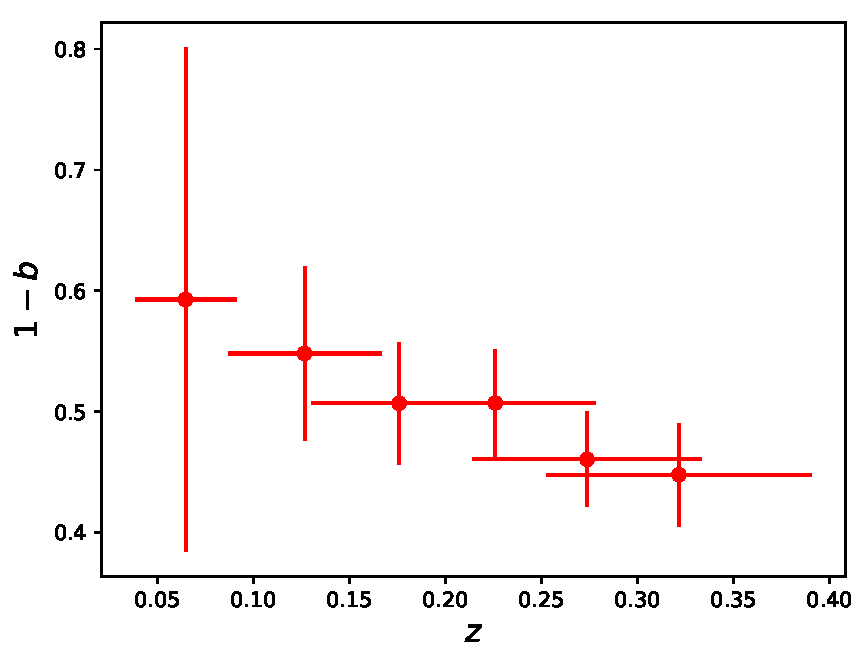
\includegraphics[width = 0.7\textwidth]{../output_test/sampler_minimal_hmc_b_hydro_all}
   \caption{Summary plot.}\label{fig:oneminusb}
  \end{figure}

\newpage
\section{Next steps}
\begin{itemize}
  \item Systematics in $gg$. We could try deprojection and see if things improve. Otherwise just remove first point or two in WISC data.
  \item Systematics in $gy$: quantify CIB contamination.
  \item Do we want a different angle on the signal modelling? E.g.:
        \begin{enumerate}
          \item Our measurement could be transformed into a measurement of the mean electron pressure weighed by halo bias at a given redshift:
                \begin{equation}
                  \bar{P}_{e,b}(z) = \int dM\,\frac{dn}{dM}\,b_h(M) \bar{P}_e(M,z)
                \end{equation}
          \item We could quantify whether there's any statistical evidence for a redshift evolution of $1-b_H$.
          \item $\rho_{gy}\simeq-0.5$. Is there anything we can say about that?
        \end{enumerate}
\end{itemize}

  
\bibliography{notes}
\bibliographystyle{habbrv}

\appendix
\section{Halo profile statistics}\label{app:hm}
  To fully account for the statistics of any halo observable, let's rederive the halo model power spectrum carefully. A given quantity $U$ at a position ${\bf x}$ is given by the cumulative effect of all halos in the universe:
  \begin{equation}
    U({\bf x})=\sum_h u_h({\bf x}-{\bf r}_h)N_h
  \end{equation}
  where the sum goes over a set of voxels covering all of space, which have been chosen to be sufficiently small so that the number of halos in each voxel, $N_h$ is either 0 or 1. ${\bf r}_h$ is the position of the halo in voxel $h$, and $u_h({\bf r})$ is the profile of $U$ around that halo.

  The Fourier transform of $U({\bf x})$ is
  \begin{align}\nonumber
    U_{\bf k}=\int dx^3\,U({\bf x})\,e^{-i{\bf k}{\bf x}}=\sum_h N_h u_h({\bf k}) e^{-{\bf r}_h{\bf k}},
  \end{align}
  where $u_h({\bf k})$ is the Fourier transform of $u_h({\bf r})$.

  Now, let's take the two-point correlator of two such fields, $U$ and $V$, in Fourier space:
  \begin{align}
    \left\langle U_{\bf k}V^*_{\bf q}\right\rangle_{p,H,\delta}&=\left\langle\sum_{h_1h_2}N_{h_1}N_{h_2}\,\left\langle u_{h_1}({\bf k})v^*_{h_2}({\bf q})\right\rangle_p\,e^{-i({\bf r}_{h_1}{\bf k}-{\bf r}_{h_2}{\bf q})}\right\rangle_{H,\delta}
  \end{align}
  Here, the subscripts $p,H,\delta$ under each ensemble average denote averaging over realizations of the profile for a given halo ($p$), over the realizations of the halo distribution ($H$) and over the realizations of the underlying dark matter distribution.

  The expression above can be rewritten as:
  \begin{align}\\
    \left\langle U_{\bf k}V^*_{\bf q}\right\rangle_{p,H,\delta}=&\left\langle\sum_h N_h\,\left\langle u_h({\bf k})v^*_h({\bf q})\right\rangle_p\,e^{-ir_h\,({\bf k}-{\bf q})}\right\rangle_{H,\delta}\\
    &+\left\langle\sum_{h_1\neq h_2}N_{h_1}N_{h_2}\,\left\langle u_{h_1}({\bf k})\right\rangle_p\left\langle v^*_{h_2}({\bf q})\right\rangle_p\,e^{-i({\bf r}_{h_1}{\bf k}-{\bf r}_{h_2}{\bf q})}\right\rangle_{H,\delta}\\
    &+\left\langle\sum_{h_1\neq h_2}N_{h_1}N_{h_2}\,{\rm Cov}\left(u_{h_1}({\bf k})v^*_{h_2}({\bf q})\right)_p\,e^{-i({\bf r}_{h_1}{\bf k}-{\bf r}_{h_2}{\bf q})}\right\rangle_{H,\delta}
  \end{align}
  Under the {\bf assumption} that the profiles for two different halos are uncorrelated, we can discard the last term, and the remaining ones are the so-called ``1-halo'' and ``2-halo'' terms.

  Let's first concentrate on the 2-halo term. Assuming that halos of mass $M$ are Poisson-distributed over the underlying halo density distribution $\delta_M({\bf x})$, the average over $H$ is equivalent to replacing $N_h$ with $\int dM\,n(M)\,dr^3_h(1+\delta_M({\bf r}_h))$, where $n(M)$ is the halo mass function. In that case we obtain:
  \begin{align}
    \left\langle U_{\bf k}V^*_{\bf q}\right\rangle_{p,H,\delta}^{2h}=&\int dM_1\,n(M_1) \langle u(k|M_1)\rangle_p\int dM_2\,n(M_2) \langle v^*(q|M_2)\rangle_p\\&\left\langle\sum_{h_1\neq h_2}dr_{h_1}^3dr_{h_2}^3(1+\delta_{M_1}({\bf r}_{h_1}))(1+\delta_{M_2}({\bf r}_{h_2}))e^{-i{\bf r}_{h_1}{\bf k}}e^{i{\bf r}_{h_2}{\bf q}}\right\rangle_{\delta},
  \end{align}
  where  we have {\bf assumed} that the only quantity that determines the statistics of halo profiles is the halo mass. Under the {\bf assumption} that the halo overdensities are deterministically related to the linear matter overdensity through a simple bias function $b(M)$ (i.e. $\delta_M({\bf x})=b(M)\delta({\bf x})$), and ignoring the unobservable ${\bf k}=0$ mode we obtain:
  \begin{align}
    \left\langle U_{\bf k}V^*_{\bf q}\right\rangle_{p,H,\delta}^{2h}=\left\langle\delta_{\bf k}\delta^*_{\bf q}\right\rangle_\delta\int dM\,n(M)\,b(M)\,\langle u(k|M)\rangle_p\,\int dM\,n(M)\,b(M) \langle v^*(q|M)\rangle_p.
  \end{align}
  Using the definition of the linear matter power spectrum ($\langle\delta_{\bf k}\delta_{\bf q}^*\rangle=(2\pi)^3\delta^{\cal D}({\bf k}-{\bf q})P_L(k)$), we obtain the final result:
  \begin{align}
    \left\langle U_{\bf k}V^*_{\bf q}\right\rangle_{p,H,\delta}^{2h}=(2\pi)^3\delta^{\cal D}({\bf k}-{\bf q})\,b_U(k)\,b_V(k)\,P_L(k),
  \end{align}
  where we have defined
  \begin{align}
    b_U(k)\equiv\int dM n(M) b(M) \left\langle u(k|M)\right\rangle_p.
  \end{align}

  Using the same approximation, the 1-halo term reads:
  \begin{align}
    \left\langle U_{\bf k}V^*_{\bf q}\right\rangle_{p,H,\delta}^{1h}&=(2\pi)^3\delta^{\cal D}({\bf k}-{\bf q})\int dM\,n(M)\,\left\langle u(k|M) v^*(k|M)\right\rangle_p\\
    &=(2\pi)^3\delta^{\cal D}({\bf k}-{\bf q})\int dM\,n(M)\,\left[\left\langle u(k|M)\right\rangle_p\left\langle v^*(k|M)\right\rangle_p+{\rm Cov}_p\left(u(k|M),v(k|M)\right)\right]
  \end{align}

  \subsection{The HOD example}
    In the case of HOD modelling of the galaxy overdensity, the galaxy density profile is modelled as:
    \begin{equation}
      u({\bf r})=n_g^{-1}\left[N_c\,\delta^{\cal D}({\bf r})+n_s({\bf r})\right],
    \end{equation}
    where $n_g$ is the total mean density of galaxies, $N_c$ is the number of central galaxies in the halo and $n_s$ is the density profile of satellite galaxies. Most commonly, $N_c$ is assumed to be either 0 or 1, and therefore has a Bernoulli distribution with probability $P(N_c=1|M)=1-P(N_c=0|M)\equiv \bar{N}_c(M)$. The satellite galaxies are usually assumed to be Poisson-distributed around a profile that is proportional to the NFW profile ($u_{\rm NFW}({\bf r}|M)$), as long as the halo already has a central galaxy. The last statement means that the number of satellite galaxies found in a differential volume element $d{\bf r}^3$ around ${\bf r}$ has a conditional distribution
    \begin{equation}
      P(n_s({\bf r})\,d{\bf r}^3=N_s|N_c,M)=
      \left\{\begin{array}{lll}
          1 & {\rm if} & N_c=0\,{\rm and}\,N_s=0\\
          0 & {\rm if} & N_c=0\,{\rm and}\,N_s>0\\
          e^{-\lambda}\frac{\lambda^{N_s}}{N_s!} & {\rm if} & N_c=1
      \end{array}\right.
    \end{equation}
    where $\lambda\equiv d{\bf r}^3\bar{N_s}(M)\,u_{\rm NFW}({\bf r}|M)$. Furthermore, the number of galaxies found in different volume elements are independent. The mean and variance of this distribution are:
    \begin{equation}
      {\rm E}(n_s({\bf r})\,d{\bf r}^3|M)={\rm Var}(n_s({\bf r})\,d{\bf r}^3|M)=d{\bf r}^3 \bar{N}_s(M)\,u_{\rm NFW}({\bf r}|M).
    \end{equation}

    Using this model, the mean Fourier profile becomes
    \begin{align}
      \langle u({\bf k})\rangle
      &=\left\langle n_g^{-1}\sum_{\bf r} d{\bf r}^3 \left[N_c\,\delta^{\cal D}({\bf r})+n_s({\bf r})\right]e^{-i{\bf k}{\bf r}}\right\rangle\\
      &=n_g^{-1}\bar{N_c}\left[1+\bar{N}_s\,u_{\rm NFW}(k|M)\right]\\
    \end{align}
    and its variance is
    \begin{align}
      \langle |u({\bf k})|^2\rangle
      &=n_g^{-2}\left\langle \sum_{\bf x} d{\bf x}^3\sum_{\bf y} d{\bf y}^3 \left[N_c\,\delta^{\cal D}({\bf x})+n_s({\bf x})\right]\,\left[N_c\,\delta^{\cal D}({\bf y})+n_s({\bf y})\right]e^{i{\bf k}({\bf y}-{\bf x})}\right\rangle\\ 
      &=n_g^{-2}\bar{N}_c\left(\left[1+\bar{N}_s\,u_{\rm NFW}({\bf k})\right]^2+\bar{N}_s\right)
    \end{align}

    So far we have ignored the total galaxy density $n_g$. This is simply given by 
    \begin{equation}
      n_g=\int dM\,n(M)\,\bar{N}_c(M)\left(1+\bar{N}_s(M)\right).
    \end{equation}
    We have also ignored the fact that we need to subtract the shot-noise contribution from the total galaxy power spectrum. This is given by $1/n_g$, which is equivalent to modifying the variance of the galaxy profile as:
    \begin{align}
      \langle |u({\bf k})|^2\rangle
      &=n_g^{-2}\left[\bar{N}_c\left(\left[1+\bar{N}_s\,u_{\rm NFW}({\bf k})\right]^2+\bar{N}_s\right)-\bar{N}_c(1+\bar{N}_s)\right]\\
      &=n_g^{-2}\bar{N}_c\left[2\bar{N}_s\,u_{\rm NFW}({\bf k})+\bar{N}_s^2u_{\rm NFW}^2({\bf k})\right]
    \end{align}

    Finally, it is easy to incorporate the fact that we may only be able to observe a fraction $f_c$ of the centrals, in which case the two profile moments read:
    \begin{align}
      \langle u({\bf k})\rangle
      &=n_g^{-1}\bar{N_c}\left[f_c+\bar{N}_s\,u_{\rm NFW}(k|M)\right]\\
      \langle |u({\bf k})|^2\rangle
      &=n_g^{-2}\bar{N}_c\left[2f_c\bar{N}_s\,u_{\rm NFW}({\bf k})+\bar{N}_s^2u_{\rm NFW}^2({\bf k})\right]
    \end{align}

\section{Translating between mass definitions}\label{app:massdef}
  We may need to translate between masses defined with different prescriptions. All of them can be described by the following equation, describing the relation between the mass and the size of a halo:
  \begin{equation}
    M_{\Delta_x}=\frac{4\pi}{3}\rho_c(z)\Delta_x\,R_{\Delta_x}^3,
  \end{equation}
  here $\Delta_x=\Delta\,f_x$, where $\Delta$ is a number (e.g. 200, 500 etc.) and $x$ is either $c$ or $m$, to distinguish between masses defined with respect to the critical density or the matter density. In either case:
  \begin{equation}
    f_c=1,\hspace{12pt} f_m=\Omega_M(z).
  \end{equation}

  Now, under the assumption that halos have an NFW density profile, it's easy to calculate the mass enclosed within a given radius:
  \begin{equation}
    M(<R)=4\pi\rho_0\,r_s^3\left[\ln\left(1+\frac{R}{r_s}\right)-\frac{R/r_s}{1+R/r_s}\right]
  \end{equation}
  Now, writing $M_{\Delta_x}=M(<R_{\Delta_x})$ and defining the concentration parameter $c_{\Delta_x}=R_{\Delta_x}/r_s$, we have, for two different mass definitions $\Delta_x$ and $\Delta'_y$:
  \begin{align}
    M_{\Delta_x}=\frac{4\pi}{3}\rho_c(z)\Delta_x\,R_{\Delta_x}^3=4\pi\rho_0\,\left(\frac{R_{\Delta_x}}{c_{\Delta_x}}\right)^3\left[\ln\left(1+c_{\Delta_x}\right)-\frac{c_{\Delta_x}}{1+c_{\Delta_x}}\right]\\
    M_{\Delta'_y}=\frac{4\pi}{3}\rho_c(z)\Delta'_y\,R_{\Delta'_y}^3=4\pi\rho_0\,\left(\frac{R_{\Delta'_y}}{c_{\Delta'_y}}\right)^3\left[\ln\left(1+c_{\Delta'_y}\right)-\frac{c_{\Delta'_y}}{1+c_{\Delta'_y}}\right].
  \end{align}
  Taking the ratio of both equations, we obtain a relation between the concentration parameters for both mass definitions:
  \begin{equation}
    \frac{c_{\Delta_x}^3\Delta_x}{c_{\Delta'_y}^3\Delta'_y}=\frac{\ln\left(1+c_{\Delta_x}\right)-\frac{c_{\Delta_x}}{1+c_{\Delta_x}}}{\ln\left(1+c_{\Delta'_y}\right)-\frac{c_{\Delta'_y}}{1+c_{\Delta'_y}}}.
  \end{equation}

  So, in order to translate between $M_{\Delta_x}$ and $M_{\Delta'_y}$:
  \begin{enumerate}
    \item Get a concentration-mass relation for $M_{\Delta_x}$ and compute both $c_{\Delta_x}$ and $R_{\Delta_x}$.
    \item Obtain $c_{\Delta'_y}$ by solving the equation above numerically.
    \item From $c_{\Delta'_y}$ obtain $R_{\Delta'_y}$ and then $M_{\Delta'_y}$.
  \end{enumerate}

\end{document}
